% ===========================================================================
\section{Design}
\label{sec:design}
% ===========================================================================

\system{} is structured around three core components: the \emph{symptom oracle},
the \emph{trial runner}, and the \emph{greedy dimensional minimizer}.
Figure~\ref{fig:architecture} shows the overall architecture.

\begin{figure}[t]
\centering
\begin{tikzpicture}[
  node distance=0.8cm and 1.2cm,
  box/.style={draw, rounded corners, minimum width=2.2cm, minimum height=0.8cm,
              font=\small, align=center},
  arrow/.style={-{Stealth[length=2mm]}, thick},
  lbl/.style={font=\scriptsize, midway, above}
]
  % Top: Input
  \node[box, fill=blue!10] (issue) {Production\\Issue};
  \node[box, fill=green!10, below=of issue] (oracle) {Symptom\\Oracle};

  % Middle: FaultForge
  \node[box, fill=orange!10, below left=0.8cm and 0.2cm of oracle] (minimizer) {Greedy\\Minimizer};
  \node[box, fill=orange!10, below right=0.8cm and 0.2cm of oracle] (runner) {Trial\\Runner};

  % Bottom: Infrastructure
  \node[box, fill=gray!10, below=1.2cm of runner] (docker) {Docker\\Cluster};
  \node[box, fill=gray!10, left=0.3cm of docker] (netem) {\texttt{tc netem}\\Injection};

  % Output
  \node[box, fill=red!10, below=1.2cm of minimizer] (recipe) {Minimal\\Recipe};

  % Arrows
  \draw[arrow] (issue) -- (oracle);
  \draw[arrow] (oracle) -- (minimizer);
  \draw[arrow] (minimizer) -- node[lbl, sloped] {\scriptsize trial} (runner);
  \draw[arrow] (runner) -- (docker);
  \draw[arrow] (netem) -- (docker);
  \draw[arrow] (docker.west) -- +(-0.5,0) |- node[font=\scriptsize, near start, right] {logs} (oracle.west);
  \draw[arrow] (minimizer) -- (recipe);
  \draw[arrow] (runner.west) -- +(-0.3,0) |- (minimizer.east);
\end{tikzpicture}
\caption{\system{} architecture. The minimizer iteratively submits trials to the
runner, which executes them against real Docker clusters with \texttt{tc netem}
fault injection. The oracle evaluates collected logs to determine reproduction,
feeding scores back to guide the binary search. The output is a minimal fault
recipe suitable for CI integration.}
\label{fig:architecture}
\end{figure}

\subsection{Symptom Oracle}
\label{sec:oracle}

The symptom oracle is a declarative specification that determines whether a
trial successfully reproduced a production issue. It provides a clean
separation between \emph{what} constitutes reproduction (domain knowledge)
and \emph{how} to find minimal triggers (search algorithm).

An oracle consists of three components:

\para{Issue metadata} Identifies the target issue: system, issue ID, title,
category (slow-fault, crash, correctness), and optional source link to the
upstream bug tracker.

\para{Validity rules} (\texttt{invalid\_if}) Conditions indicating infrastructure
failure rather than system behavior. If Docker Compose fails to start, or the
benchmark crashes before fault injection, the trial is \emph{invalid} and
excluded from scoring. This prevents the minimizer from converging on
configurations that simply break the test harness.

\para{Reproduction rules} (\texttt{reproduced\_if}) Log patterns indicating
the target symptom was triggered. Rules support:
\begin{itemize}[leftmargin=*,topsep=2pt,itemsep=1pt]
  \item \texttt{contains}: Exact substring match in specified log file.
  \item \texttt{regex}: Regular expression match with capture groups.
  \item \texttt{any}: Disjunction (any matching rule suffices).
  \item \texttt{all}: Conjunction (all rules must match).
  \item Nested groups for complex logic.
\end{itemize}

\begin{lstlisting}[language={},caption={Example oracle for etcd Raft election.},label={lst:oracle}]
issue:
  id: "ETCD-RAFT-ELECTION"
  system: "etcd"
  title: "Leader election cascade under
          network delay"
  source: "github.com/etcd-io/etcd/issues/18109"
  category: "slow-fault"

invalid_if:
  any:
    - file: info
      contains: "docker-compose up failed"

reproduced_if:
  any:
    - file: compose
      regex: "raft.*elected leader"
    - file: compose
      regex: "the leader changed"
    - file: compose
      regex: "elected.*term"

severity_threshold: 1
\end{lstlisting}

\para{Scoring} The oracle returns a score $s \in [0, 1]$ computed as:
\begin{equation}
s = \min\left(\frac{|\text{matched signals}|}{\text{severity\_threshold}}, 1.0\right)
\end{equation}

The minimizer uses $s \geq 0.5$ as the reproduction threshold ($\theta$). This
provides robustness against transient log noise: a trial that matches some but
not all expected signals is still considered reproducing if it exceeds half the
threshold. We evaluate oracle precision and recall in Section~\ref{sec:oracle-eval}.

\subsection{Trial Model}
\label{sec:trial-model}

A \emph{trial} is the atomic unit of execution: a complete specification of
system configuration, workload, and fault injection.

\begin{equation}
\text{Trial} = \langle \text{System}, \text{Benchmark}, \text{Faults} \rangle
\end{equation}

\noindent where:
\begin{align}
\text{System} &= \langle \text{name}, \text{version}, \text{cluster\_size} \rangle \\
\text{Benchmark} &= \langle \text{name}, \text{exec\_time\_s} \rangle \\
\text{Fault} &= \langle \text{type}, \text{location}, \text{severity}, \text{duration}, \text{start} \rangle
\end{align}

Each fault is parameterized by five dimensions:
\begin{itemize}[leftmargin=*,topsep=2pt,itemsep=1pt]
  \item \textbf{type} $\in$ \{nw, fs, cpu, mem, process\}: The fault class.
  \item \textbf{location}: Target node identifier (\eg{}, ``leader'', ``node1'').
  \item \textbf{severity}: Fault intensity, type-specific (\eg{},
        \texttt{slow-5ms} for network, \texttt{cpus-0.25} for CPU).
  \item \textbf{duration}: Injection time in seconds.
  \item \textbf{start}: Delay before injection begins (seconds after benchmark start).
\end{itemize}

A trial with multiple faults ($|\text{Faults}| > 1$) enables testing of
\emph{fault interactions}, \eg{}, simultaneous network delay on two nodes, or
combined network + filesystem degradation on a single node.

\subsection{Greedy Dimensional Minimizer}
\label{sec:minimizer}

The minimizer is \system{}'s key algorithmic contribution. Given a reproducing
trial $T_0$ (where the oracle confirms the symptom), it iteratively reduces
fault parameters to find $T_{\min}$, a locally minimal trial that still
reproduces.

\begin{algorithm}[t]
\caption{Greedy Dimensional Minimization}
\label{alg:minimizer}
\begin{algorithmic}[1]
\Require Reproducing trial $T_0$, oracle $O$, budget $B$
\Ensure Locally minimal reproducing trial $T_{\min}$
\State $T \gets T_0$
\Statex
\State \Comment{\textbf{Phase 1: Reduce fault count}}
\For{$i = |T.\text{faults}|$ \textbf{downto} 1}
  \State $T' \gets T$ with fault $i$ removed
  \If{$O(\text{run}(T')) \geq \theta$}
    \State $T \gets T'$ \Comment{fault $i$ unnecessary}
  \EndIf
\EndFor
\Statex
\State \Comment{\textbf{Phase 2: Minimize severity (binary search)}}
\For{each remaining fault $f_i \in T.\text{faults}$}
  \State $lo \gets 0, \; hi \gets \text{magnitude}(f_i.\text{severity})$
  \For{$k = 1$ \textbf{to} $B_{\text{mag}}$}
    \State $mid \gets (lo + hi) / 2$
    \State $T' \gets T$ with $f_i.\text{severity} \gets \text{build}(mid)$
    \If{$O(\text{run}(T')) \geq \theta$}
      \State $hi \gets mid$ \Comment{can go lower}
    \Else
      \State $lo \gets mid$ \Comment{too low, go higher}
    \EndIf
  \EndFor
  \State $T \gets T$ with $f_i.\text{severity} \gets \text{build}(hi)$
\EndFor
\Statex
\State \Comment{\textbf{Phase 3: Minimize duration (binary search)}}
\For{each fault $f_i \in T.\text{faults}$}
  \State Binary search over $[1, f_i.\text{duration\_s}]$
  \State Update $f_i.\text{duration\_s} \gets \text{min found}$
\EndFor
\Statex
\State \Comment{\textbf{Phase 4: Maximize start time (binary search)}}
\For{each fault $f_i \in T.\text{faults}$}
  \State Binary search over $[f_i.\text{start\_s}, \text{max\_start}]$
  \State Update $f_i.\text{start\_s} \gets \text{max found that reproduces}$
\EndFor
\State \Return $T$
\end{algorithmic}
\end{algorithm}

\para{Phase ordering} The phases are ordered by expected impact: fault count
reduction eliminates entire faults (largest effect), severity reduction
narrows the primary parameter, duration reduction shortens exposure time, and
timing optimization finds the latest trigger point. This greedy ordering
maximizes reduction per trial spent.

\para{Correctness invariant} The algorithm maintains the invariant that $T$
always reproduces (oracle score $\geq \theta$) at each phase boundary. Binary
search within a phase may temporarily produce non-reproducing candidates (when
$lo$ increases), but the final value ($hi$) is always reproducing.

\para{Complexity} For a trial with $k$ faults and budget parameters
$B_{\text{mag}}, B_{\text{dur}}, B_{\text{time}}$:
\begin{equation}
\text{Total iterations} \leq k + k \cdot (B_{\text{mag}} + B_{\text{dur}} + B_{\text{time}}) + 1
\end{equation}

With default configuration ($B_{\text{mag}}=8$, $B_{\text{dur}}=5$,
$B_{\text{time}}=5$) and a single-fault trial ($k=1$), the maximum is 19
iterations. Empirically we observe 17--18 (the initial verification trial
uses 1 iteration, and phases that converge early return budget to later phases).

\para{Precision guarantee} After $B_{\text{mag}}$ binary search steps over
range $[0, S_{\max}]$, the converged severity satisfies:
\begin{equation}
|s_{\text{converged}} - s_{\text{true}}| \leq \frac{S_{\max}}{2^{B_{\text{mag}}}}
\end{equation}

For $S_{\max} = 5000$\,ms and $B_{\text{mag}} = 8$: precision = 19.5\,ms.
For the same budget from $S_{\max} = 10000$\,ms (Redis): precision = 39\,ms.
This precision is a \emph{configurable} property: operators trade iterations
for tighter bounds.

\begin{figure}[t]
\centering
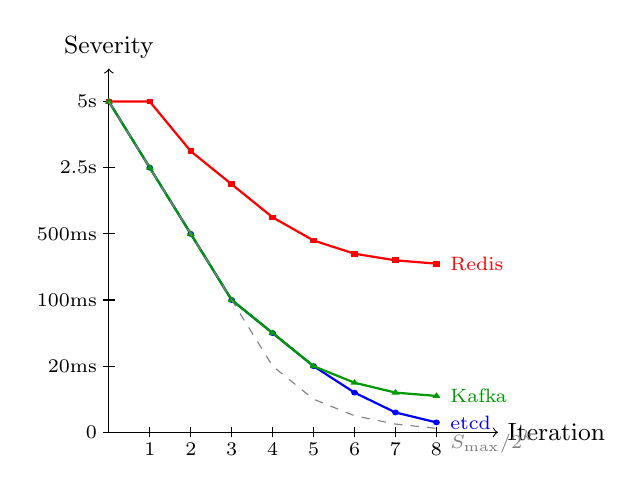
\begin{tikzpicture}[
  xscale=0.52, yscale=0.42,
]
% Axes
\draw[->] (0,0) -- (9.5,0) node[right, font=\small] {Iteration};
\draw[->] (0,0) -- (0,11) node[above, font=\small] {Severity};

% Y-axis labels (log-like spacing mapped to linear for clarity)
\foreach \y/\lbl in {0/0, 2/20ms, 4/100ms, 6/500ms, 8/2.5s, 10/5s} {
  \draw (-0.15,\y) -- (0.15,\y) node[left=3pt, font=\scriptsize] {\lbl};
}
% X-axis labels
\foreach \x in {1,...,8} {
  \draw (\x,-0.15) -- (\x,0.15) node[below=2pt, font=\scriptsize] {\x};
}

% etcd convergence (boundary ~19.5ms, very low)
% hi values: 5000, 2500, 1250, 625, 312.5, 156.3, 78.1, 39.1, 19.5
\draw[blue, thick, mark=*,mark size=1.5pt] plot coordinates {
  (0,10) (1,8) (2,6) (3,4) (4,3) (5,2) (6,1.2) (7,0.6) (8,0.3)
};
\node[blue, font=\scriptsize, right] at (8.1,0.3) {etcd};

% Redis convergence (boundary ~2700ms from 10s range)
% hi: 10000, 10000, 7500, 6250, 5000, 3750, 3125, 2812, 2700
\draw[red, thick, mark=square*,mark size=1.5pt] plot coordinates {
  (0,10) (1,10) (2,8.5) (3,7.5) (4,6.5) (5,5.8) (6,5.4) (7,5.2) (8,5.1)
};
\node[red, font=\scriptsize, right] at (8.1,5.1) {Redis};

% Kafka convergence (boundary ~78ms)
% hi: 5000, 2500, 1250, 625, 312.5, 156.3, 78.1, 78.1, 78.1
\draw[green!60!black, thick, mark=triangle*,mark size=1.5pt] plot coordinates {
  (0,10) (1,8) (2,6) (3,4) (4,3) (5,2) (6,1.5) (7,1.2) (8,1.1)
};
\node[green!60!black, font=\scriptsize, right] at (8.1,1.1) {Kafka};

% Dashed line showing exponential convergence envelope
\draw[gray, dashed, thin] plot coordinates {
  (0,10) (1,8) (2,6) (3,4) (4,2) (5,1) (6,0.5) (7,0.25) (8,0.12)
};
\node[gray, font=\scriptsize, right] at (8.1,-0.3) {$S_{\max}/2^k$};

\end{tikzpicture}
\caption{Convergence of the severity binary search for three representative
systems. The $hi$ bound (current upper bound on boundary) decreases
exponentially. etcd and Kafka converge to the precision floor; Redis converges
to its true boundary at 2.7\,s. The dashed line shows the theoretical
$S_{\max}/2^k$ envelope.}
\label{fig:convergence}
\end{figure}

\para{Monotonicity assumption} Binary search requires that the oracle response
is monotone with severity: if $O(s) = \text{reproduced}$, then
$\forall s' > s: O(s') = \text{reproduced}$. We validate this assumption
empirically (Section~\ref{sec:monotonicity}) and discuss conditions under which
it may be violated (Section~\ref{sec:limitations}).

\subsection{Noise-Tolerant Probing}
\label{sec:probing}

At boundary severities, distributed systems exhibit non-deterministic behavior:
the same trial may reproduce on one run but not the next due to timing
variability in leader election, gossip convergence, or thread scheduling. A
na\"ive binary search that makes one evaluation per midpoint can converge on a
non-reproducing value due to a single unlucky trial.

\system{} addresses this through a \emph{composable probe strategy} that
separates noise-handling policy from the search algorithm. The minimizer
delegates all reproduction decisions to an injected strategy:

\begin{itemize}[leftmargin=*,topsep=2pt,itemsep=1pt]
  \item \textbf{SingleShotProbe}: One evaluation per decision. Fast ($O(1)$
        overhead) but vulnerable at noisy boundaries. Used when the system is
        known to be deterministic (\eg{}, consensus systems far from their
        boundary).
  \item \textbf{MajorityVoteProbe}: Evaluates $k$ times (default $k=3$) and
        requires a supermajority ($\geq 66\%$) to declare reproduction. This
        provides $1 - \binom{k}{\lceil k \cdot p \rceil} p^{\lceil k \cdot p
        \rceil}$ false-positive resilience where $p$ is the transient
        reproduction rate below boundary.
\end{itemize}

The strategy is injected via a protocol interface, so custom strategies
(\eg{}, adaptive repetition that increases $k$ near boundaries) can be added
without modifying the minimizer.

\para{Post-convergence boundary validation} After binary search converges at
severity $hi$ (the lowest value that reproduced), \system{} optionally runs a
\emph{boundary validator} that dense-probes both $hi$ and $lo$ (the highest
value that did not reproduce) with $n$ additional trials each. This produces a
\emph{validated boundary interval}:

\begin{equation}
\text{BoundaryInterval} = \langle lo, hi, r_{above}, r_{below}, c \rangle
\end{equation}

\noindent where $r_{above}$ and $r_{below}$ are measured reproduction rates at
$hi$ and $lo$ respectively, and $c = r_{above} - r_{below}$ is the
\emph{confidence separation}. A clean boundary shows $r_{above} \approx 1.0$,
$r_{below} \approx 0.0$, and $c \approx 1.0$. We report confidence separation
for all converged boundaries in Section~\ref{sec:eval}.

\subsection{Search Strategy Layer}
\label{sec:search}

Before minimization, \system{} needs a reproducing trial as input. The
\emph{search} layer provides this by exploring the fault parameter space:

\begin{itemize}[leftmargin=*,topsep=2pt,itemsep=1pt]
  \item \textbf{Exhaustive grid}: Cartesian product of all parameter values,
        tested in lexicographic order.
  \item \textbf{Shuffled grid}: Same space, randomized traversal order to
        avoid systematic bias.
  \item \textbf{Random subset}: Uniform random sample from the full grid,
        bounded by a trial budget.
\end{itemize}

In practice, operators typically know a high-severity configuration that
reproduces (\eg{}, ``5\,s delay always triggers election''). \system{}'s
minimizer starts from this known-good configuration, eliminating the need for
an initial search phase in most use cases.

\subsection{Multi-Fault Minimization}
\label{sec:multi-fault}

For trials with multiple simultaneous faults, Phase~1 (fault count reduction)
attempts to eliminate each fault while preserving reproduction. This identifies
which faults are \emph{necessary} for the symptom and which are redundant.

The interaction effects of multi-fault trials create a non-trivial search
problem: fault $A$ alone may not reproduce, fault $B$ alone may not reproduce,
but $A + B$ together may reproduce through interaction. \system{}'s greedy
approach handles this correctly; it only removes a fault if the remaining
faults still reproduce, preserving necessary interactions.

After count reduction, the per-fault binary search in Phases 2--4 minimizes
each remaining fault independently. This produces a locally minimal multi-fault
recipe: no single fault can be further reduced without losing reproduction.
